\documentclass[12pt, letterpaper]{article}
\usepackage{ifxetex}
\usepackage{verbatim} %for comment environment

\usepackage{fullpage} %sane margins
%\usepackage{ulem} %strikeouts?
\usepackage{amsmath} %mathematics
%\usepackage{amssymb} %more maths, but conflicts with SIunits :C
\usepackage{graphicx} %GOOD GRAPHICS
\usepackage{subfig, wrapfig}
\usepackage{SIunits} %units
\usepackage{euler} %whoa! smexy!
%for specifying fonts

%xetex-specific font directives
\ifxetex %cm-default makes equations not look like shit if euler isn't loaded
\usepackage[cm-default]{fontspec}% provides font selecting commands
\usepackage{xunicode}% provides unicode character macros
\usepackage{xltxtra} % provides some fixes/extras
\setmainfont{Times New Roman}
\fi

\title{Determining Anisotropic Thermal Conductivity of Snow With Needle Probe Measurements}
\author{Joshua Holbrook}
\date{\today}

\begin{document}

\maketitle

\begin{abstract}
The thermal conductivity of snow is an important factor in climate models because it determines the energy exchange between the earth's soil and its atmosphere.However, it is difficult to measure due to snow's porous, anisotropic nature. I propose to simulate the measurement of thermal conductivity in anisotropic snow with needle probes numerically in order to develop a method for ascertaining the actual thermal conductivity from multiple needle probe measurements. Then, this method will be tested against materials of known anisotropy to test the predictions of the model. Finally, the method will be used to collect actual thermal conductivity measurements of snow. This will allow scientists to accurately characterize the thermal conductivity of natural snow and to monitor change in conductivity over time. This will enable more accurate climate modeling for arctic regions.
\end{abstract}

%\pagebreak

\section{Introduction and Background}

During the long arctic winters, snow's thermal behavior plays a critical role in determining the net energy exchange between the earth's surface and its atmosphere. This energy exchange is an important factor in local and regional arctic climate models. The thermal conductivity of snow is highly dependent on its layered, anisotropic structure and density (figure \ref{fig:snow}). Snow changes structure over time, mostly due to self-weight settlement and the transport of water vapor within the snow \cite{sturm2}. This vapor transport happens because the temperature gradients across snow cause varying vapor pressures within the snow. This causes ice to sublime into water vapor at warmer areas with higher vapor pressure, and recondense into ice at cooler areas with lower vapor pressure (figure \ref{fig:snow}c).

\begin{figure}[h]
\centering
\caption{Mechanisms for the Development of Anisotropy in Snow}
\label{fig:snow}
\subfloat[][Fresh snowfall settles rapidly, creating an anisotropic density gradient.]{\includegraphics[width=1.6in]{snow_1}}\quad
\subfloat[][Cool air and warm soil cause a temperature differential across the snow.]{\includegraphics[width=1.6in]{snow_2}}\quad
\subfloat[][Due to these differences in vapor pressure and buoyancy effects, ice sublimes from lower sections of the snow layer and deposits at regions closer to the surface, creating a gradient in snow structure (depth hoar).]{\includegraphics[width=1.6in]{snow_3}}\\
\subfloat[][Also, sintering of discrete ice crystals, conglomerating due to vapor transport, diffusion effects and even freeze-thaw events can form layers.]{\includegraphics[width=1.6in]{snow_5}}\quad
\subfloat[][The end result is the development of discrete layers in the snow with their own structures and density gradients, resulting in anisotropic thermal conductivity.]{\includegraphics[width=1.6in]{snow_4}}\quad
\subfloat[][Often, fresh snow adds yet another layer of snow and the snowscape grows even more complex.]{\includegraphics[width=1.6in]{snow_6}}
\end{figure}

At the same time, this vapor transport combined with diffusion and freeze-thaw effects cause discrete snow crystals to fuse together, creating solid connections between snow particles (figure \ref{fig:snow}d). In the typical case that the surrounding air (hence the upper layer of snow) is warmer than the ground (and the lower layers of snow), upper areas in the snow layer will become relatively solid and lower reaches of the snow will remain tenuously connected at best---in other words, the snow will form a crust (figure \ref{fig:snow}e).  Conduction in snow happens primarily through solid ice connections, in contrast to conducting through air pockets. As a consequence, high-density snow conducts more readily than low-density snow and well-sintered snow conducts more readily than depth hoar. The snow has highly anisotropic thermal properties as a whole. Of course, the conductivity properties of snow continue to change over time, as temperature gradients change (due to warm periods, temperature inversions and the arrival of Spring) and as fresh, less-conductive snowfall adds even more layering to the snow cover (figure \ref{fig:snow}f). What all this means is that the very energy exchange that depends on the thermal conductivity of snow has a drastic effect on this same conductivity.

The importance of quantifying the thermal conductivity of snow has been known for quite some time, leading to a significant amount of work based on a wide variety of data and theories \cite{sturm3,conductivitymodels}. Some of these are based on the microscale, working with the thermal behavior of individual snow particles, while others work on a much larger scale, relating overall thermal conductivity of snow to such variables as density, temperature, and even the age of snow \cite{mustructure2,sturm1}.  While the basis for these conductivity models vary widely and snow is surprisingly difficult to properly characterize, scientists are slowly arriving at a concensus regarding the isotropic thermal properties of snow as functions of snow type and density. However, while the thermal properties of homogenous snow may be well-characterized, there remains a critical gap between these properties and those of the anisotropic snow that is found in a natural snowpack.

\begin{wrapfigure}{L}{0.44\textwidth}
\centering
\label{fig:needleprobe}
\includegraphics[width=0.4\textwidth]{simple.png}
\caption{A COMSOL model of a needle probe in snow. The cube represents a block of snow, while the needle probe itself appears as a thin line running part-way down the middle.}
\end{wrapfigure}

To bridge this gap, scientists must make on-site field measurements of snow's thermal conductivity. Typically, this is done with a needle probe, which has the advantage of being able to make measurements while preserving the structure of the fragile snow. This is in contrast to the guarded hot-plate method, which instead sandwiches a material between two plates of differing temperatures; The guarded hot-plate method, unlike the needle probe method, requires a sample to be removed from its environment and placed into a box-like apparatus.

A needle probe consists of a thin metal rod embedded with an electric heating element and either a thermistor or thermocouple (figure 2). The heat element generates a constant amount of heat, and the high thermal conductivity of metal causes the entire needle to have a uniform temperature distribution. The needle is inserted into the material and the temperature of the needle is measured over time. %note \ref{fig:needleprobe} wasn't working

For uniform, isotropic materials, the thermal conductivity can be ascertained by approximating the needle as a line (of infinite length) and solving the governing equations for transient heat conduction in cylindrical coordinates for temperature as a function of time \cite{probetheory}. After a sufficiently long amount of time, this equation converges on the following \cite{werc}:

\begin{equation*}
T(r,t) = \frac{Q}{4\pi k}\ln(t) + c(r)
\end{equation*}

where \(T\) is temperature, \(t\) is time, \(Q\) is heat flow per length of the probe. This solution indicates that, after some initial transient behavior (the longevity of which is effected by the thermal diffusivity of the needle's surroundings), the thermal conductivity of the substance is directly proportional to the slope of the temperature as a function of the natural logarithm of time (figure 3) \cite{probetheory}.
Needle probes have been very successful in measuring the thermal conductivity of many isotropic materials, including soils, reconstituted snow, and even food. Commercial needle probes are widely available; however, being designed for measuring the thermal conductivity of soils, they are shorter than is ideal for snow (since the lower thermal conductivity of snow makes the infinite line source assumption less valid) and assume less transient behavior than snow offers (due to air on the snow/needle boundary causing a higher apparent thermal diffusivity). Comparing measurements taken by needle probes with those using the guarded hot-plate method indicates that both techniques are accurate for measuring isotropic materials with uniform properties in the ranges they were designed for. However, the situation is different with anisotropic materials. %note \ref{fig:loggraph} wasn't working

\begin{wrapfigure}{R}{0.42\textwidth}
\centering
\label{fig:loggraph}
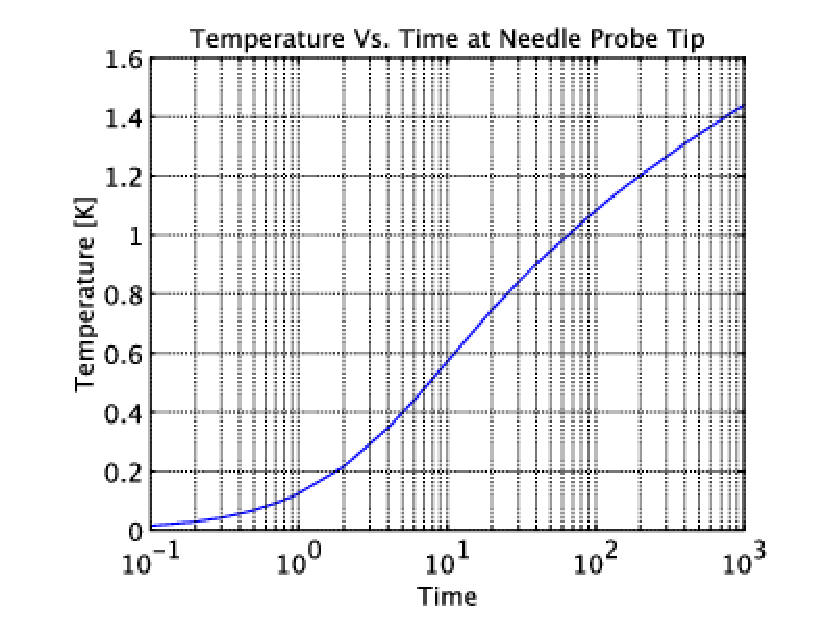
\includegraphics[width=0.4\textwidth]{lolg_scale}
\caption{When plotting \(T\) vs. \(\ln(t)\) of a needle probe, the slope of the linear portion may be used to calculate the heat conductivity of an isotropic medium.}
\end{wrapfigure}

In contrast with the needle probe, the guarded hot-plate imposes a one-dimensional temperature gradient on a material in rectangular coordinates. As such, it is commonly believed to be the only device which can measure the thermal conductivity of anisotropic materials. Even then, the guarded hot-plate method can measure anisotropy in only one direction, and additionally requires that the direction of anisotropy be known beforehand such that the direction may be aligned with the temperature gradient in the device. Using this technique to measure the thermal conductivity of snow is very difficult, since the technique would require that samples be extracted from their location, transported to the lab and properly oriented into the guarded hot-plate. This must all be done without changing the structure of the snow through disturbance from moving it, or through a continuation over time, of the same mechanisms that cause snow to metamorphose in nature. Because needle probes allow for relatively non-disturbing in-situ measurements, being able to use them in the case of anisotropic snow would overcome these difficulties.

There have been some successes in the past with measuring other anisotropic materials with needle probes. In particular, researchers in Germany adopted a needle probe method to measure thermal conductivity of stone collected from a pilot borehole for the KBT superdeep well in Oberpfalz, West Germany \cite{ktb}. For this application, the researchers cut smooth faces into their samples and pressed their needle probes onto the surface. By taking many measurements and plotting the measured conductivities as a function of direction, they found the extreme conductivities along these faces. While their method relies on more measurements than we would like and was used on a very different material, their study suggests that anisotropic conductivity measurements with needle probes is also possible for our case.

\section{Objectives and Methodology}

I propose to investigate the feasibility of using the needle probe method to determine the anisotropic thermal conductivity of snow by using needle probes inserted in multiple directions. The major objective for this project is three-fold:  First, numerical modeling shall be used to develop a methodology for measuring anisotropic heat conductivity using needle probes. Then, the results will be experimentally corroborated in the laboratory using materials of known, engineered anisotropy. Finally the method will be tested in-situ on snow.

\subsection{Numerical Modeling}

In the simplest case, and the most familiar one to many, steady-state purely conductive heat transfer is characterized by the following governing equation for one-dimensional heat conduction:

\begin{equation*}
\dot{Q}=-kA\frac{dT}{dx}
\end{equation*}\\

In this case, \(k\) is a scalar property. However, for systems with two or even three dimensions, the governing equation becomes more complex:

\begin{equation*}
\vec{q}=-K \nabla \vec{T}
\end{equation*}

In this equation, \(\vec{q}\) is heat flux (for example, \(\watt \per \square \meter\) ), and \(\nabla \vec{T}\) is temperature gradient. More notable is that instead of a scalar \(k\), this equation has a symmetric and positive definite matrix \(K\) which encodes anisotropic properties of the material (if the material is in fact isotropic, \(K\) would be a multiple of the identity matrix (that is, \(K=kI\)), making it exactly equivalent to \(k\)).

%Will be useful, but needs to be relocated
%\begin{comment}
\begin{wrapfigure}{L}{0.44\textwidth}
\centering
\label{fig:isotherms}
\includegraphics[width=0.4\textwidth]{isotherms}
\caption{The same COMSOL model as in figure 2 has been solved. The surfaces plotted in this visualization represent isotherms in the snow after the needle probe has operated for a "long time." The needle probe itself appears as a thin line running down the middle.}
\end{wrapfigure}
%\end{comment}

COMSOL and MATLAB will be used to model the behavior of needle probe readings in materials of varying anisotropy and at varying angles with respect to the material's orientation (figure 4). From this data, we intend to develop a method for solving for \(K\) based on a minimum amount of measurements.


%\begin{comment}
\begin{wrapfigure}{Rb}{0.42\textwidth}
\centering
\label{fig:m_ellipsoid}
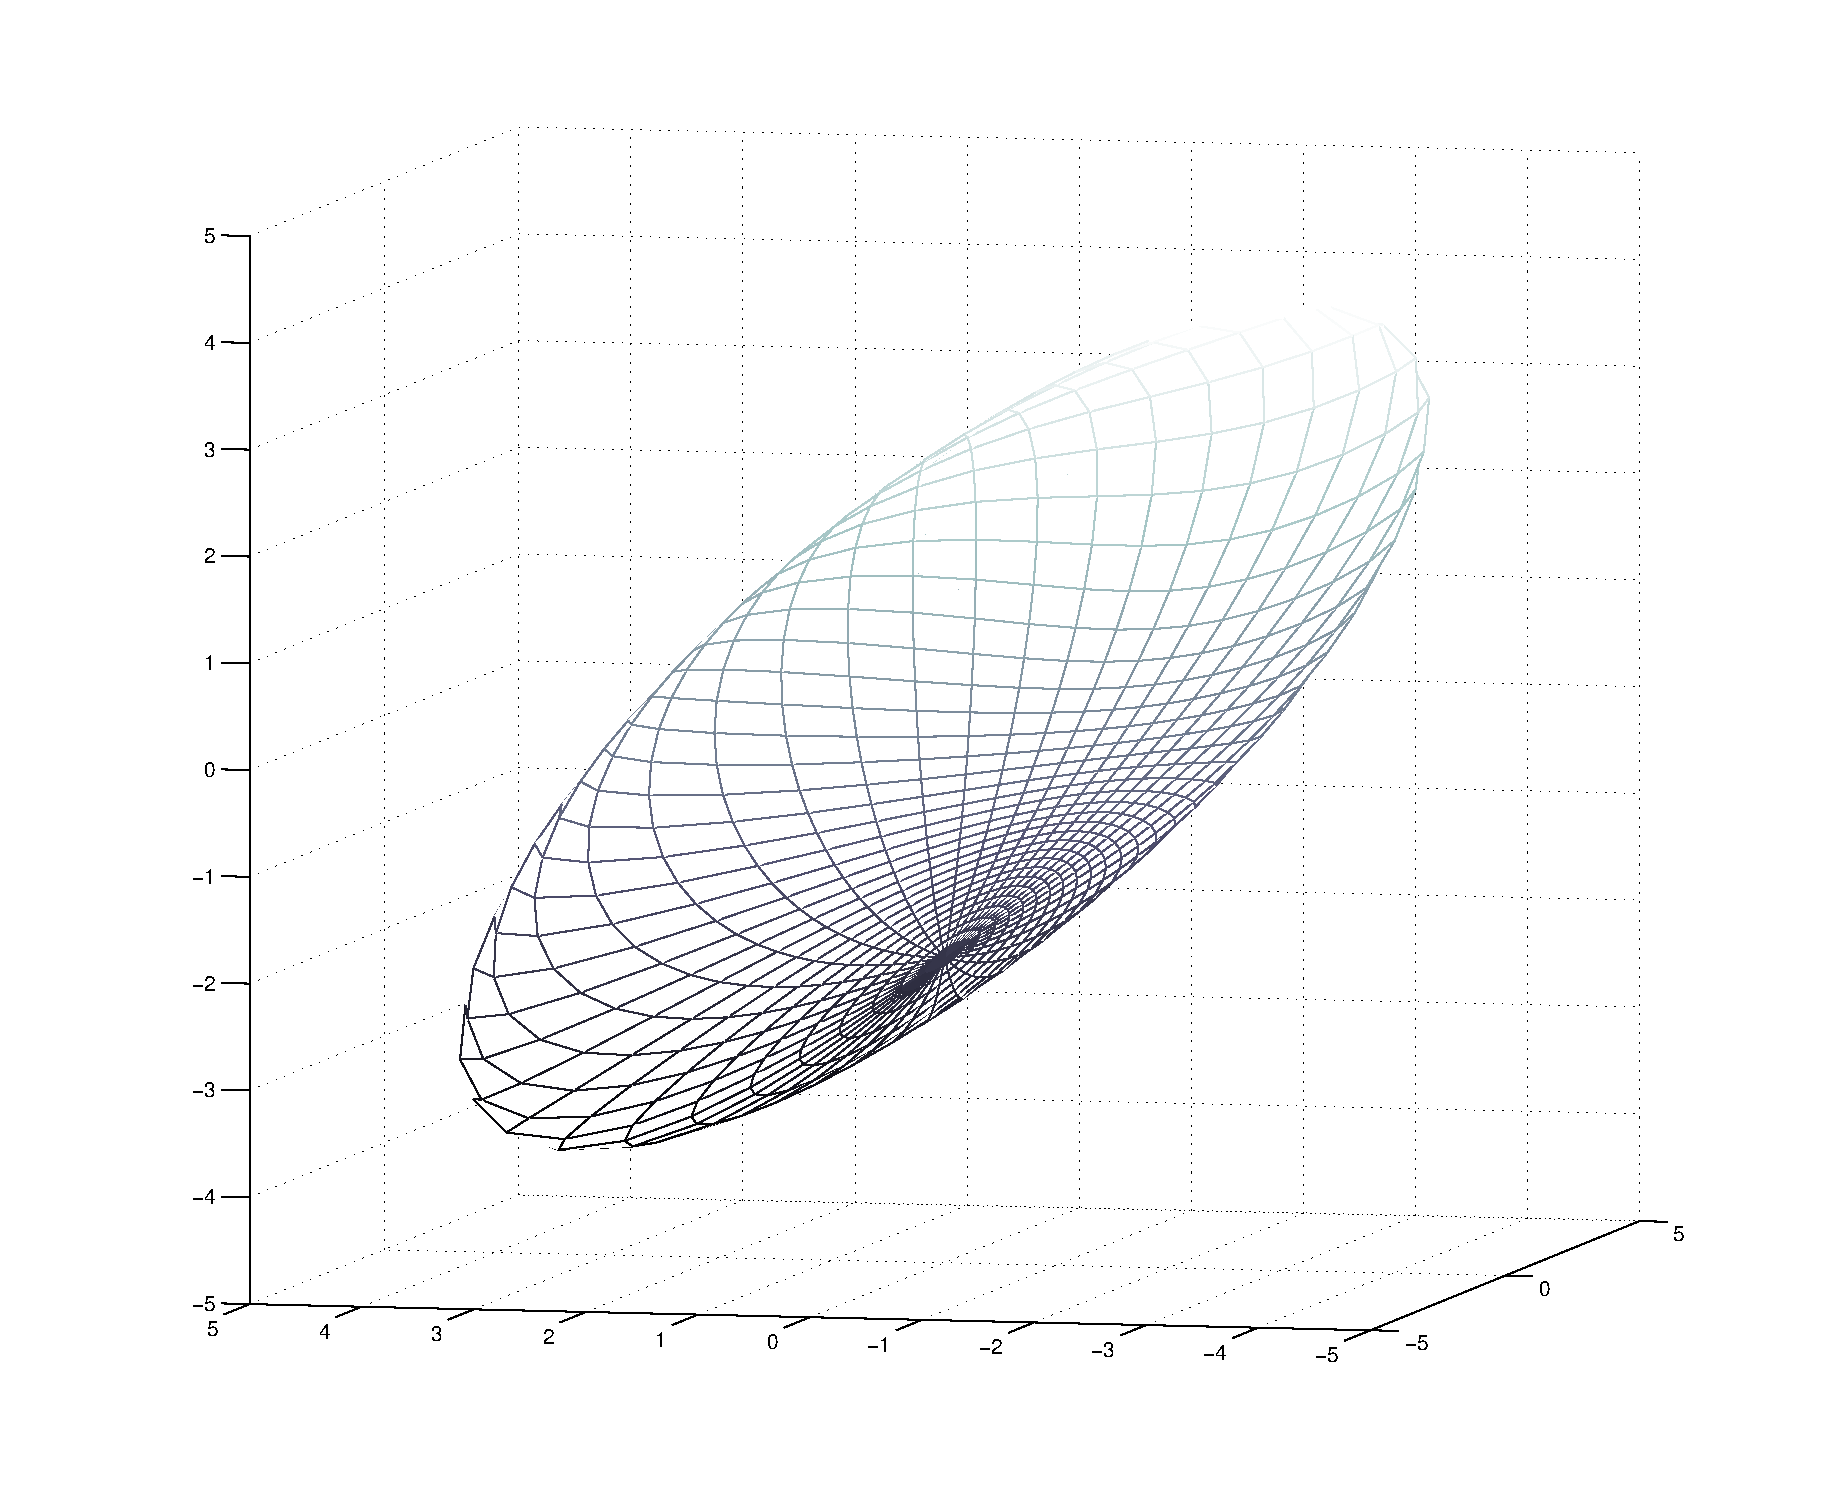
\includegraphics[width=0.4\textwidth]{m_ellipsoid}
\caption{One way to visualize a symmetric, positive-definite matrix such as \(K\) is to plot the ellipsoid \(\vec{x}^TK\vec{x}=1\). The length of a vector \(\vec{x}\) which satisfies this equation is equal to \(1/\sqrt{k}\) for the effective thermal conductivity \(k\) in that direction.}
%\vspace{-72pt}
\end{wrapfigure}
%\end{comment}

One idea for being able to find the conductivity matrix \(K\) is to use an ellipsoid equation. If the directions of anisotropy are aligned with the \(\vec{x}, \vec{y}\) and \(\vec{z}\) directions, then the equation as related to anisotropic conductivity would look like this:

\begin{equation*}
\left(\frac{x}{k_x}\right)^2 + \left(\frac{y}{k_y}\right)^2 + \left(\frac{z}{k_z}\right)^2 = 1
\end{equation*}

If the effective thermal conductivity \(k\) is determined for a given direction, then if \(x,y\) and \(z\) are chosen so that they are in the same direction but \(x^2 + y^2 +z^2 = (1/k)^2\) instead of simply \(k\), these values can be substituted into the above equation to limit what the constants \(k_x, k_y\) and \(k_z\) can be. If this is done for enough directions, then one can solve for \(k_x, k_y\) and \(k_z\).

Of course, this particular method means that the directions of anisotropy must be known a'priori. So, instead, a more flexible, but more complicated, equation for an ellipsoid must be used (Figure 5):

\begin{equation*} \vec{x}^TK\vec{x}=1 \end{equation*}

This equation works similar to the previous one. However, it can be used to solve for any given \(K\), as long as it's symmetrical. The same technique may be used to solve for \(K\), if the effective thermal conductivity can be determined in enough directions. Because \(K\) is \(3 \times 3\) (for three dimensions) and is symmetrical, this means that \(K\) has six unknowns. This suggests that six effective heat conductivities, and hence measurements, will be required to find \(K\).


\subsection{Experimental Corroboration}

Once we have a mathematical model for the material, we will test it in the laboratory. We will assemble composite materials of known anisotropy, made with alternating layers of materials with higher and lower heat conductivity. Examples of composites include paper and aluminum foil, foamboard and ice, and foamboard and silicone compound.

Needle probes will be inserted into these composites and readings will be collected for multiple directions within them. We will also take conductivity measurements with a guarded hot-plate apparatus. The results from the custom needle probes, the commercial needle probe and the guarded hot-plate will be compared to each other. We will have data on how well our needle probe method fares against a hot-plate method, and benchmarks for the commercial needle probes as compared to the guarded hot-plate and our custom needle probes.

\subsection{Field Application Testing}

Finally, once the method is proven in the laboratory, it shall be used in the field to measure the anisotropic thermal conductivity properties of actual snow in the field. Much as will be the case with the artificial composites, needle probe measurements will be taken of snow, from which anisotropy profiles of real snow will be calculated.

We will use permanently-installed needle probes to measure the thermal conductivity of snow throughout the season in multiple locations. We expect to see the properties of snow to be fairly isotropic early in the year, and become more anisotropic as winter wears on. While we won't realistically be able to test snow in a guarded hot-plate apparatus for comparison, seeing the trends we expect from theory, in addition to the laboratory experiments, will validate our method. We will not only have hard data on snow anisotropy, but will also have supporting evidence of whether our method works.

If the use of commercial needle probes seems viable based on laboratory experiments, we will also once again compare the measurements of commercial needle probes with those of custom needle probes. This will act as a definitive test for the reliability of commercial needle probes for anisotropic snow conductivity measurements.

\pagebreak
%references, thx bibtex
\nocite{*}
\bibliographystyle{Science}
\bibliography{proposal}

\pagebreak

\section*{Project Schedule}
\begin{center}
\begin{tabular}{r | l}
Date & Event\\
\hline
May 15th, 2010 & Preliminary results of COMSOL modeling tabulated\\
July 15th, 2010 & Method for finding conductivity matrix \(K\) formulated\\
September 15th, 2010 & Laboratory testing of developed method ready to begin\\
December 1st, 2010 & Laboratory testing of developed method complete\\
February 1st, 2011 & Initial measurements of snow conductivity collected\\
March 15th, 2011 & Results compiled and papers written
\end{tabular}
\end{center}

\section*{Budget}
\begin{center}
\begin{tabular}{r | r}
Item & Cost\\
\hline
Graduate student PI summer stipend & \$5,000\\
Travel to a conference & \$1,500\\
Publication fees & \$200\\
Commercial needle probes & \$500\\
Data acquisition equipment & \$500\\
Equipment and materials for laboratory measurements & \$500\\
\textbf{TOTAL} & \textbf{\$8,800}
\end{tabular}
\end{center}

\section*{Budget Justification}
\$5,000 as stipend for the student PI is requested to support his research over the summer. \$1,500 is requested for travel to a conference to report on the student PI's findings to the AGU or other relevant organization.  Moreover, \$200 is requested to pay for publishing fees with AGU or other relevant publisher. \$500 is requested for the purchase of commercial needle probes from Decagon for testing purposes and another \$500 is requested for the purchase of data acquisition equipment to use with the needle probes. \$500 is also requested to fund construction of anisotropic materials, custom needle probes and any other small-scale apparatus required to conduct laboratory experiments.

\end{document}
